\section{Introduction}
Pathology foundation models (FMs) provide diverse histological representations learned from large-scale WSI datasets \citep{conchv1andconchv15,gigapath,hibou,hoptimus0,hoptimus1,midnight12k,phikon,phikonv2,univ1anduniv2,virchow,virchow2}.
However, these models are trained under heterogeneous paradigms, yielding varied representations.

Nevertheless, no single pathology foundation model universally dominates all clinical diagnostic tasks \citep{boutaj2026from,vanderbilt2026goldmark}.
This limitation raises a critical challenge: how to effectively integrate heterogeneous foundation model representations.
Although different foundation models provide diverse feature views of WSI data, simply increasing the number of integrated models or applying naive fusion strategies does not necessarily improve fusion performance.

Existing fusion approaches, including feature concatenation, attention-based methods \citep{vaswani2017attention}, and mixture-of-experts (MoE) routing \citep{shazeer2017moe}, have explored increasingly adaptive mechanisms for integrating representations.
However, the relationship between foundation-model representation characteristics and downstream fusion behavior remains insufficiently understood.

\begin{figure}[htbp]
    \centering
    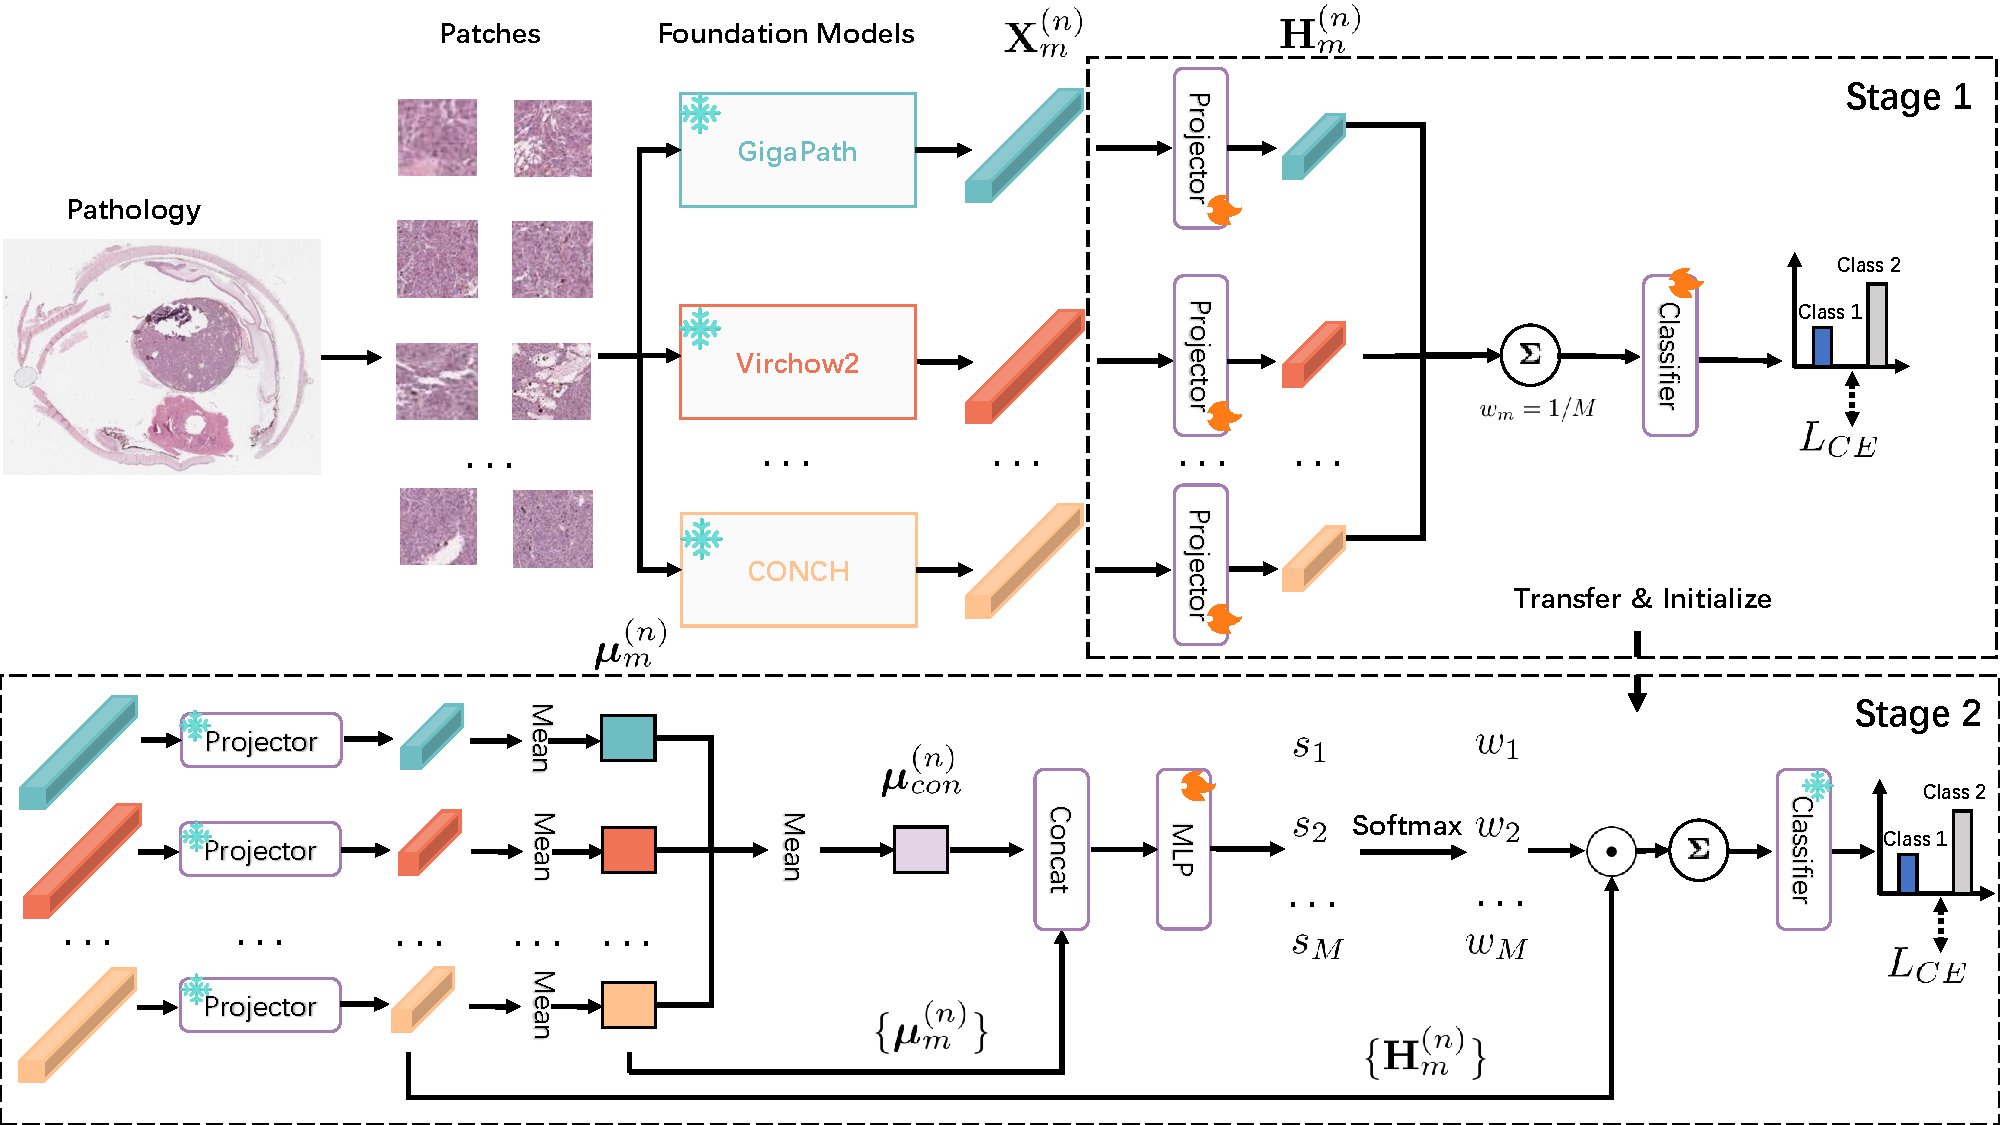
\includegraphics[width=1.0\linewidth]{figs/um_fm/main figure.pdf}
    \caption{Overview of CoR-Fuse. Stage 1 initializes projection heads and the downstream classifier with mean fusion, while Stage 2 uses a consensus representation for adaptive routing. For slide $n$ and foundation model $m$, patch representations $\mathbf{X}_m^{(n)}$ are projected to $\mathbf{H}_m^{(n)}$ and mean-pooled into $\mathbf{\mu}_m^{(n)}$. CoR-Fuse produces one set of slide-level routing weights, shared across all patch embeddings to preserve the spatial bag structure, and is compatible with MIL, MLP, and GNN downstream architectures.}
    \label{fig:main_figure}
\end{figure}

In this work, we formulate multi-FM fusion as estimating sample-specific encoder contributions to the downstream task, rather than applying fixed weights.
Each foundation model may contribute useful information, but its relative contribution can vary across models and samples.
To better understand the underlying factors affecting multi-foundation-model fusion, we establish a systematic analysis framework that investigates foundation model relationships from three perspectives.

On TCGA-UVM, through systematic analyses based on this three-perspective framework, we derive several insightful observations:
1. Fusion effectiveness varies with foundation-model composition rather than the number of integrated models alone.
2. Representation similarity alone does not reliably indicate whether an encoder contributes redundant or complementary task-relevant information.
3. No single fusion strategy consistently dominates, the relative effectiveness of fusion strategies varies with the composition of the integrated representations.
4. Per-model marginal contribution is sample-dependent, with substantial variation across slides.

Driven by these key insights, we further develop CoR-Fuse (Consensus-aware Routing Fusion), a lightweight, plug-and-play routing module for multi-foundation-model fusion that combines encoder-specific representations with cross-encoder consensus to estimate task-adaptive encoder weights through a two-stage optimization strategy (Figure~\ref{fig:main_figure}).
CoR-Fuse constructs a fused representation compatible with downstream architectures, including multiple instance learning (MIL) \citep{ilse2018abmil}, graph neural networks (GNNs) \citep{gnn} and MLP-based classifiers.
We extensively evaluate CoR-Fuse across multiple TCGA cohorts \citep{tcga}, investigating its robustness under different foundation-model compositions, fusion strategies, and computational settings.

Our main contributions are summarized as follows:

\begin{itemize}
\item We identify model-specific and sample-specific variation in encoder contributions in multi-foundation-model fusion.

\item We develop a three-perspective analysis of representation geometry, feature association, and task-level contribution, suggesting that representation similarity alone does not fully characterize functional redundancy or fusion behavior.

\item We show that CoR-Fuse provides competitive predictive performance while exhibiting lower empirical composition-level performance dispersion across the evaluated encoder compositions, suggesting more consistent behavior under changes in foundation-model composition.
\end{itemize}
